\documentclass{article}
\usepackage[T1]{fontenc}
\usepackage[utf8]{inputenc}

% Language setting
% Replace `english' with e.g. `spanish' to change the document language
% Idioma sin shorthands conflictivos para bibpunct
\usepackage[spanish,es-noshorthands]{babel} 
\spanishdecimal.
% Set page size and margins
% Replace `letterpaper' with`a4paper' for UK/EU standard size
\usepackage[letterpaper,top=2cm,bottom=2cm,left=3cm,right=3cm,marginparwidth=1.75cm]{geometry}

% Useful packages
\usepackage{amsmath}
\usepackage{graphicx}
\usepackage{float}
\usepackage{times}
\usepackage{natbib}
\usepackage[colorlinks=true, allcolors=blue]{hyperref}
\usepackage{geometry}
\usepackage{graphics}
%\usepackage[sf,bf,tiny,center,compact]{titlesec}
\usepackage{subfigure}
\usepackage{tabularx}
\usepackage{amssymb}
\usepackage{mathrsfs}
\usepackage{hyphenat}
\usepackage{tikz}
\usepackage{blox}
\hyphenation{co-mer-cial rea-li-zan si-guien-te si-mu-la-ción ke-lly con-si-de-ra-da}
\AtBeginDocument{\bibpunct{(}{)}{;}{a}{,}{,}}

%Variables Comúnes:
\newcommand{\EstudianteA}{Calli Yereki Peña Pérez}
\newcommand{\EstudianteB}{Aaron Emmanuel Trejo Jotolín}
\newcommand{\EstudianteC}{Dani}
\newcommand{\EstudianteD}{Kevini}
\newcommand{\EstudianteE}{Ivancini}
\newcommand{\EstudianteF}{Dieguini}
\newcommand{\NumeroPractica}{67}
\newcommand{\TituloPractica}{LonemInsumLONenISu}
\newcommand{\FechaCompromiso}{67 de mayo de 6767}
\newcommand{\FechaEntrega}{\today}

\begin{document}

%portada
\begin{titlepage}
\centering
	\begin{figure}
  \begin{minipage}{1\linewidth}
     \centering\centering%\rule{2cm}{2cm}
    % \caption{Primera figura}
    
\includegraphics[width=0.3\textwidth]{img/logos_fi_uaq.png}
     
  \end{minipage}
\end{figure}
{\scshape\LARGE Universidad Autónoma de Querétaro \par}
	\vspace{0.5cm}
	{\scshape\Large Facultad de Ingeniería \par}
	\vspace{0.5cm}
	{\scshape\Large Ingeniería en Automatización \par}
	\vspace{0.5cm}	
	{\Large\bfseries Control II\par}
	\vspace{0.8cm}
	{\Large\bfseries \TituloPractica \\ \par}	
	\vspace{0.8cm}
	{\Large\itshape Práctica \NumeroPractica\par}
	\vspace{0.8cm}
	Profesor: \par
	Dr. Roberto Valentín Carrillo Serrano \par
	\vspace{0.5cm}
	Equipo 1\par \vspace{0.2cm}
	Integrantes:\vspace{0.4cm}
\par	
	\EstudianteA \hfill \rule{70mm}{0.1mm}
\vspace{0.4cm}
\par    
    \EstudianteB \hfill \rule{70mm}{0.1mm}
\vspace{0.4cm}
\par
    \EstudianteC \hfill \rule{70mm}{0.1mm}
\vspace{0.4cm}
\par
    \EstudianteD \hfill \rule{70mm}{0.1mm}
\vspace{0.4cm}
\par
    \EstudianteE \hfill \rule{70mm}{0.1mm}
\vspace{0.4cm}
\par
    \EstudianteF \hfill \rule{70mm}{0.1mm}

\par
	
		
	\vfill

% Bottom of the page
	{\large Fecha compromiso: \FechaCompromiso\par
    Fecha en que se entregó: \FechaEntrega}.
\end{titlepage}

%\frontmatter	%fija la numeración romana
\thispagestyle{empty}%no imprimir número de página en índice
\tableofcontents
\listoffigures
\listoftables
%\printindex
\newpage
%\setcounter{page}{1}
%\mainmatter 	%fija la numeración arábiga



\section{Objetivo}
Controlar posición de la flecha de un motor de CD con escobillas usando un controlador discreto por asignación de polos cumpliendo condiciones de diseño especificadas en una función de transferencia discreta deseada.

\section{Marco Teórico}
La transformada de Laplace se define del siguiente modo. Suponga que se tiene una función del tiempo $f(t)$, la transformada de Laplace de $f(t)$ se representa por $F(s)$, es decir $\mathscr{L}\{f(t)\}=F(s)$ y se puede calcular como \citep{Ogata2010}:
\begin{equation}
\mathscr{L}\{f(t)\}=F(s)=\int_{0}^{\infty}f(t)e^{-st}dt
\label{eq:Def-Laplace}
\end{equation}

La relación que existe entre la entrada y la salida se muestra en \eqref{eq:FTmotor}:
\begin{equation}
G(s)=\frac{Y(s)}{U(s)}=\frac{150}{s\left( s+\sqrt{\frac{2}{x_\alpha}} \right) }
\label{eq:FTmotor}
\end{equation}
donde se aprecia que \eqref{eq:FTmotor} tiene una ``raíz'' en el origen y otra ``raíz'' en $s=-\sqrt{\frac{2}{x_\alpha}}$ (ver la apertura y cierre de comillas en LaTeX) por lo que el sistema en \eqref{eq:FTmotor} es inestable \citep{HernandezBook2013}. Observar que en referencias cruzadas a ecuación se usa el comando \emph{\textbackslash eqref} para que quede entre paréntesis el número de ecuación (favor de respetar la sangría al inicio de un nuevo párrafo, es decir, después de un punto y aparte).

\cite{Aguado2003} consideran a la estabilidad como el primer objetivo del control automático.

El primer objetivo del control automático es la estabilidad y como segundo objetivo se tiene que el error en estado estacionario sea cero \citep{Aguado2003}. No olvidar que $g=9.81\left[\frac{m}{s^2}\right]$ (las unidades van entre corchetes y con un espacio entre el valor numérico y la apertura de los mismos).

La expresión (respetar el espacio matemático entre ecuaciones como en \eqref{eq:U}) para la energía potencial es \citep{Aguado2000}:
\begin{equation}
U=mgh,\quad h=l_1+\frac{1}{2}l_0%Espacio matemático con \quad
\label{eq:U}
\end{equation}

El modelo dinámico no lineal del péndulo con dos ruedas obtenido con las ecuaciones de Euler-Lagrange está dado por \citep{HernandezBook2024}:
\begin{equation}
M(q)\ddot{q}+C(q,\dot{q})\dot{q}+g(q)=B(q)\tau
\label{eq:Mod_comp}
\end{equation}
\begin{equation}
q=[x_o\quad y_o\quad \theta\quad \alpha\quad \phi_r\quad \phi_l]^T
\label{eq:q}
\end{equation}
\begin{equation}
M(q)=\begin{bmatrix}
M_p(1+\tan^2{(\beta)}) & 0 & \Delta_1 & \Delta_2 & 0 & 0\\ 
0 & M_p & \Delta_3 & \Delta_4 & 0 & 0\\
\Delta_1 & \Delta_3 & \Delta_5 & 0 & 0 & 0\\
\Delta_2 & \Delta_4 & 0 & M_pC_z^2+I_{yy} & 0 & 0\\
0 & 0 & 0 & 0 & M_wR^2+I_{wa} & 0\\
0 & 0 & 0 & 0 & 0 & M_wR^2+I_{wa}
\end{bmatrix}
\label{eq:M}
\end{equation}

\begin{equation}
\Delta_1=-M_pC_z\sin(\alpha)\sin(\theta)
\label{eq:Delta1}
\end{equation}

Para ecuaciones grandes o multilínea:
\begin{multline}
p(x) = [3x^6 + 14x^5y + 590x^4y^2 + 19x^3y^3\\ 
- 12x^2y^4 - 12xy^5 + 2y^6 - a^3b^3+1087b^6 +a-2b+1030c-7d]
\label{eq:p_de_x}
\end{multline}



\section{Materiales y Métodos}
Esta plantilla base para reportes funciona con el programa miktex como compilador y con el visualizador texmaker (ambos gratuitos en internet).

Las características del sistema se pueden ver reflejadas en el Cuadro \ref{tabla:carac_pic} del cual se pueden extraer las funcionalidades iniciales. Se ajusta el periodo de muestreo para evitar el fenómeno de \textit{aliasing} conocido también en idioma español como solapamiento. Las unidades se reportan en el Sistema Internacional $(SI)$, van entre corchetes en formato matemático con un espacio entre el valor y la apertura de corchetes.
\begin{table}[H]
\centering
\caption{Características del PIC18F4431 \citep{HernandezBook2013}.} 
\begin{tabular}{|c|c|}\hline
Características: & Cantidad y/o valor $[unidad\ SI]$: \\ \hline
Pines totales & 40\\
PWM's & 8\ de\ $14\ [b]$\\
Velocidad máxima & $40\ [MHz]$\\
Memoria flash & $16\ [kB]$\\
Memoria EEPROM & $256\ [B]$\\
RAM estática & $768\ [B]$\\
Pines de Entradas/salidas & 36\\
Distancia entre pines & $2.52\ [mm]$\\
Temporizadores & 1 de $8\ [b]$, 3 de $16\ [b]$\\
Módulos para leer encoder & 1\\ \hline
\end{tabular}
\label{tabla:carac_pic}
\end{table}

Respecto a las herramientas generales de inteligencia artificial (IA):

\begin{enumerate}
\item Se permite el uso de estas herramientas con el propósito de apoyo para la revisión de la redacción.

\item La o las personas que utilicen estas herramientas son responsables de la redacción y asumen las consecuencias de los errores, lo anterior debido a que los resultados de estas herramientas pueden ser: no actualizados, incompletos, incorrectos y/o sesgados.

\item Los autores son, en última instancia responsables, y además, responsables del contenido del trabajo.

\item No se permite el uso de herramientas generativas de IA para crear o alterar imágenes en reportes. Esto puede incluir mejorar, oscurecer, moverse, eliminar o introducir una característica específica dentro de una imagen o figura. Los ajustes de brillo, contraste o equilibrio de color son aceptables si no oscurecen ni eliminan ninguna información presente en el original.

\item Si algún autor del reporte llegara a usar alguna herramienta de IA es necesario que en las conclusiones individuales se exprese las secciones del reporte en que fue utilizada, qué tipo de IA se uso, cómo se usó y para qué se usó.

\item En caso de que software especializado o el profesor encuentren que se uso la IA en algunas partes del reporte y los autores responsables lo especificaron en las conclusiones individuales: si esto sucede en una sección colectiva, al equipo completo se le descontarán 0.5 puntos por ocurrencia. En caso de que ocurra en una sección individual el miembro o los miembros que incurran en este caso se les descontarán 0.5 puntos por ocurrencia en el trabajo. 

\item En caso de que software especializado o el profesor encuentren que se uso la IA en algunas partes del reporte y los autores responsables no lo especificaron en las conclusiones individuales: si esto sucede en una sección colectiva, al equipo completo se le descontarán 2 puntos por ocurrencia. En caso de que ocurra en una sección individual el miembro o los miembros que incurran en este caso se les descontarán 2 puntos por ocurrencia en el trabajo. 

\end{enumerate} 

Para Cuadros con expresiones matemáticas en su interior:
\begin{table}[H]
\centering
\caption{Controladores clásicos con la aproximación bilineal \citep{notasclase}.}
\label{tab:controladores-bilineal}
\begin{tabular}{|c|c|c|}
\hline
Regulador:    & $G(s)$: & $G(z)$: \\ \hline
PD                    &$G(s)=k\left[1+T_vs\right]$&$G(z)\approx k\frac{\left[1+\frac{2T_v}{T}\right]+\left[1-\frac{2T_v}{T}\right]z^{-1}}{1+z^{-1}}$\\ \hline
PI                    &$G(s)=k\left[1+\frac{1}{T_ns}\right]$&$G(z)\approx k\frac{\left[1+\frac{T}{2T_n}\right]+\left[\frac{T}{2T_n}-1\right]z^{-1}}{1-z^{-1}}$\\ \hline
PID                   &$G(s)=k\left[1+\frac{1}{T_ns}+T_vs\right]$&\begin{tabular}[c]{@{}c@{}}$G(z)\approx\frac{a_0+a_1z^{-1}+a_2z^{-2}}{1-z^{-2}}$\\$a_0=k\left[1+\frac{T}{2T_n}+\frac{2T_v}{T}\right]$\\$a_1=k\left[\frac{T}{T_n}-\frac{4T_v}{T}\right]$\\$a_2=k\left[\frac{T}{2T_n}+\frac{2T_v}{T}-1\right]$\end{tabular}\\ \hline
Redes &$G(s)=k\left[\frac{1+\tau_1s}{1+\tau_2s}\right]$&$G(z)\approx k\frac{\left[1+\frac{2\tau_1}{T}\right]+\left[1-\frac{2\tau_1}{T}\right]z^{-1}}{\left[1+\frac{2\tau_2}{T}\right]+\left[1-\frac{2\tau_2}{T}\right]z^{-1}}$\\ \hline
\end{tabular}
\end{table}

Para poner diagramas de bloques se utiliza la paquetería ``blox'' (observar en el código los comandos que se usan para apertura y cierre de comillas), la cual cuenta con herramientas detalladas sobre como realizar diferentes diagramas. Para lograr que funcione es necesario agregar la paquetería al proyecto, así como en el preámbulo del documento mandar llamar los paquetes ``tikz'' y ``blox''. Aquí un ejemplo sencillo (ver Figura \ref{fig:LRsimple}): 

    \begin{figure}[H]
    \centering
        \begin{tikzpicture}[scale=1.0, transform shape]
            \bXInput{A}
            \bXComp[5]{B}{A}
            \bXLink[$R(s)$]{A}{B}
            \bXBloc[2]{C}{$\frac{1}{s+c_1}$}{B}
            \bXLink[$E(s)$]{B}{C}
            \bXOutput{E}{C}
            \bXLink[$Y(s)$]{C}{E}
            \bXReturn{C-E}{B}{}
        \end{tikzpicture}
        \caption{Lazo de retroalimentación simple \citep{notasclase}.}
        \label{fig:LRsimple}
    \end{figure}


En la Figura \ref{fig:EjercicioBloques} se muestra un diagrama de bloques con varios lazos de retroalimentación:

    \begin{figure}[H]
    \centering
        \begin{tikzpicture}[scale=1.0, transform shape]
            \bXInput{A}
            \bXCompSum[5]{B}{A}{}{-}{+}{}
            \bXLink[$R(s)$]{A}{B}
            \bXCompSum[3]{C}{B}{}{+}{+}{}
            \bXLink{B}{C}
            \bXBloc[2]{D}{$G_1(s)$}{C}
            \bXLink{C}{D}
            \bXCompSum[4]{E}{D}{-}{}{+}{}
            \bXLink{D}{E}
            \bXBloc[2]{F}{$G_2(s)$}{E}
            \bXLink{E}{F}
            \bXBloc[2]{G}{$G_3(s)$}{F}
            \bXLink{F}{G}
            \bXOutput[4]{H}{G}
            \bXLink[]{G}{H}
            \bXLinkName[.6]{H}{$Y(s)$}
            \bXBranchy[-3.5]{G}{I}
            \bXBlocr[2]{J}{$H_2(s)$}{I}
            \bXLinkyx{G-H}{J}
            \bXLinkxy{J}{E}
            \bXBranchy[3.5]{F}{K}
            \bXBlocr[2]{L}{$H_1(s)$}{K}
            \bXLinkyx{F-G}{L}
            \bXLinkxy{L}{C}
            \bXReturn[6]{G-H}{B}{}
        \end{tikzpicture}
        \caption{Diagrama de bloques con varios lazos de retroalimentación.}
        \label{fig:EjercicioBloques}
    \end{figure}

    \begin{figure}[H]
    \centering
        \begin{tikzpicture}[scale=0.5, transform shape]
            \bXInput{A}
            \bXCompSum[5]{B}{A}{}{-}{+}{}
            \bXLink[$R(s)$]{A}{B}
            \bXCompSum[3]{C}{B}{}{+}{+}{}
            \bXLink{B}{C}
            \bXBloc[2]{D}{$G_1(s)$}{C}
            \bXLink{C}{D}
            \bXCompSum[4]{E}{D}{-}{}{+}{}
            \bXLink{D}{E}
            \bXBloc[2]{F}{$G_2(s)$}{E}
            \bXLink{E}{F}
            \bXBloc[2]{G}{$G_3(s)$}{F}
            \bXLink{F}{G}
            \bXOutput[4]{H}{G}
            \bXLink[]{G}{H}
            \bXLinkName[.6]{H}{$Y(s)$}
            \bXBranchy[-3.5]{G}{I}
            \bXBlocr[2]{J}{$H_2(s)$}{I}
            \bXLinkyx{G-H}{J}
            \bXLinkxy{J}{E}
            \bXBranchy[3.5]{F}{K}
            \bXBlocr[2]{L}{$H_1(s)$}{K}
            \bXLinkyx{F-G}{L}
            \bXLinkxy{L}{C}
            \bXReturn[6]{G-H}{B}{}
        \end{tikzpicture}
        \caption{Diagrama de bloques con varios lazos de retroalimentación a la mitad de tamaño.}
        \label{fig:EjercicioBloquesmitad}
    \end{figure}
    



\section{Resultados y Discusión}
Se ponen los Cuadros y/o Figuras que muestran los resultados producto de de la práctica o de la implementación. Es necesario discutirlos tanto de manera individual como colectiva.

En la Figura \ref{fig:sim} se presenta la respuesta temporal en simulación del sistema en lazo cerrado cuando se controla la posición de la flecha de salida del motor de CD.

\begin{figure}[H]
	\centering
		
\includegraphics[width=0.30\textwidth]{img/logos_fi_uaq.png}
	\caption{Escudos.}
	\label{fig:Escudos}
\end{figure}

En la Figura \ref{fig:Escudos} se muestran los escudos con escala de $0.3$ (equivalente al $30\ [\%]$ del tamaño del renglón).

\begin{figure}[H]
	\centering
		
\includegraphics[width=0.60\textwidth]{img/logos_fi_uaq.png}
	\caption{Escudos al doble de tamaño y sin salirse de la caja.}
	\label{fig:Escudos-doble}
\end{figure}

Para que las gráficas de simulación en simulink tengan el mismo formato que las gráficas experimentales, se utiliza el bloque \textit{To workspace} (ver Figura \ref{fig:diagsim}), así con los datos de la simulación que se generan en el espacio de trabajo de matlab, se puede crear un archivo txt correspondiente a la simulación y correr un código semejante al que hace la gráfica experimental (ver Anexo \ref{proggsim}) con el intérprete de LaTeX asegurando el mismo formato tanto en las gráficas de simulación como en las gráficas experimentales.

\begin{figure}[H]
	\centering
		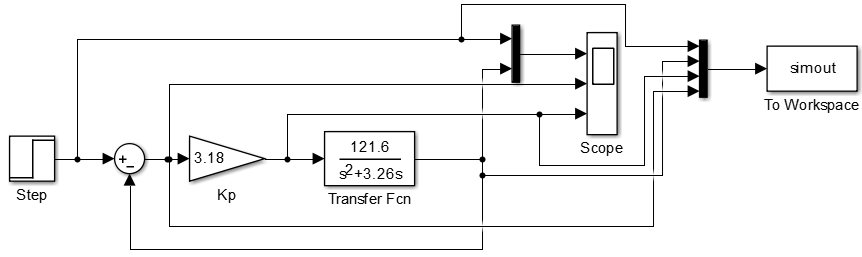
\includegraphics[width=0.97\textwidth]{img/diag_simulink.png}
	\caption{Diagrama para simulación del sistema en lazo cerrado con $K_p=3.18$ para $r=\pi\ [rad]$ en simulink.}
	\label{fig:diagsim}
\end{figure}

\begin{figure}[H]
	\centering
		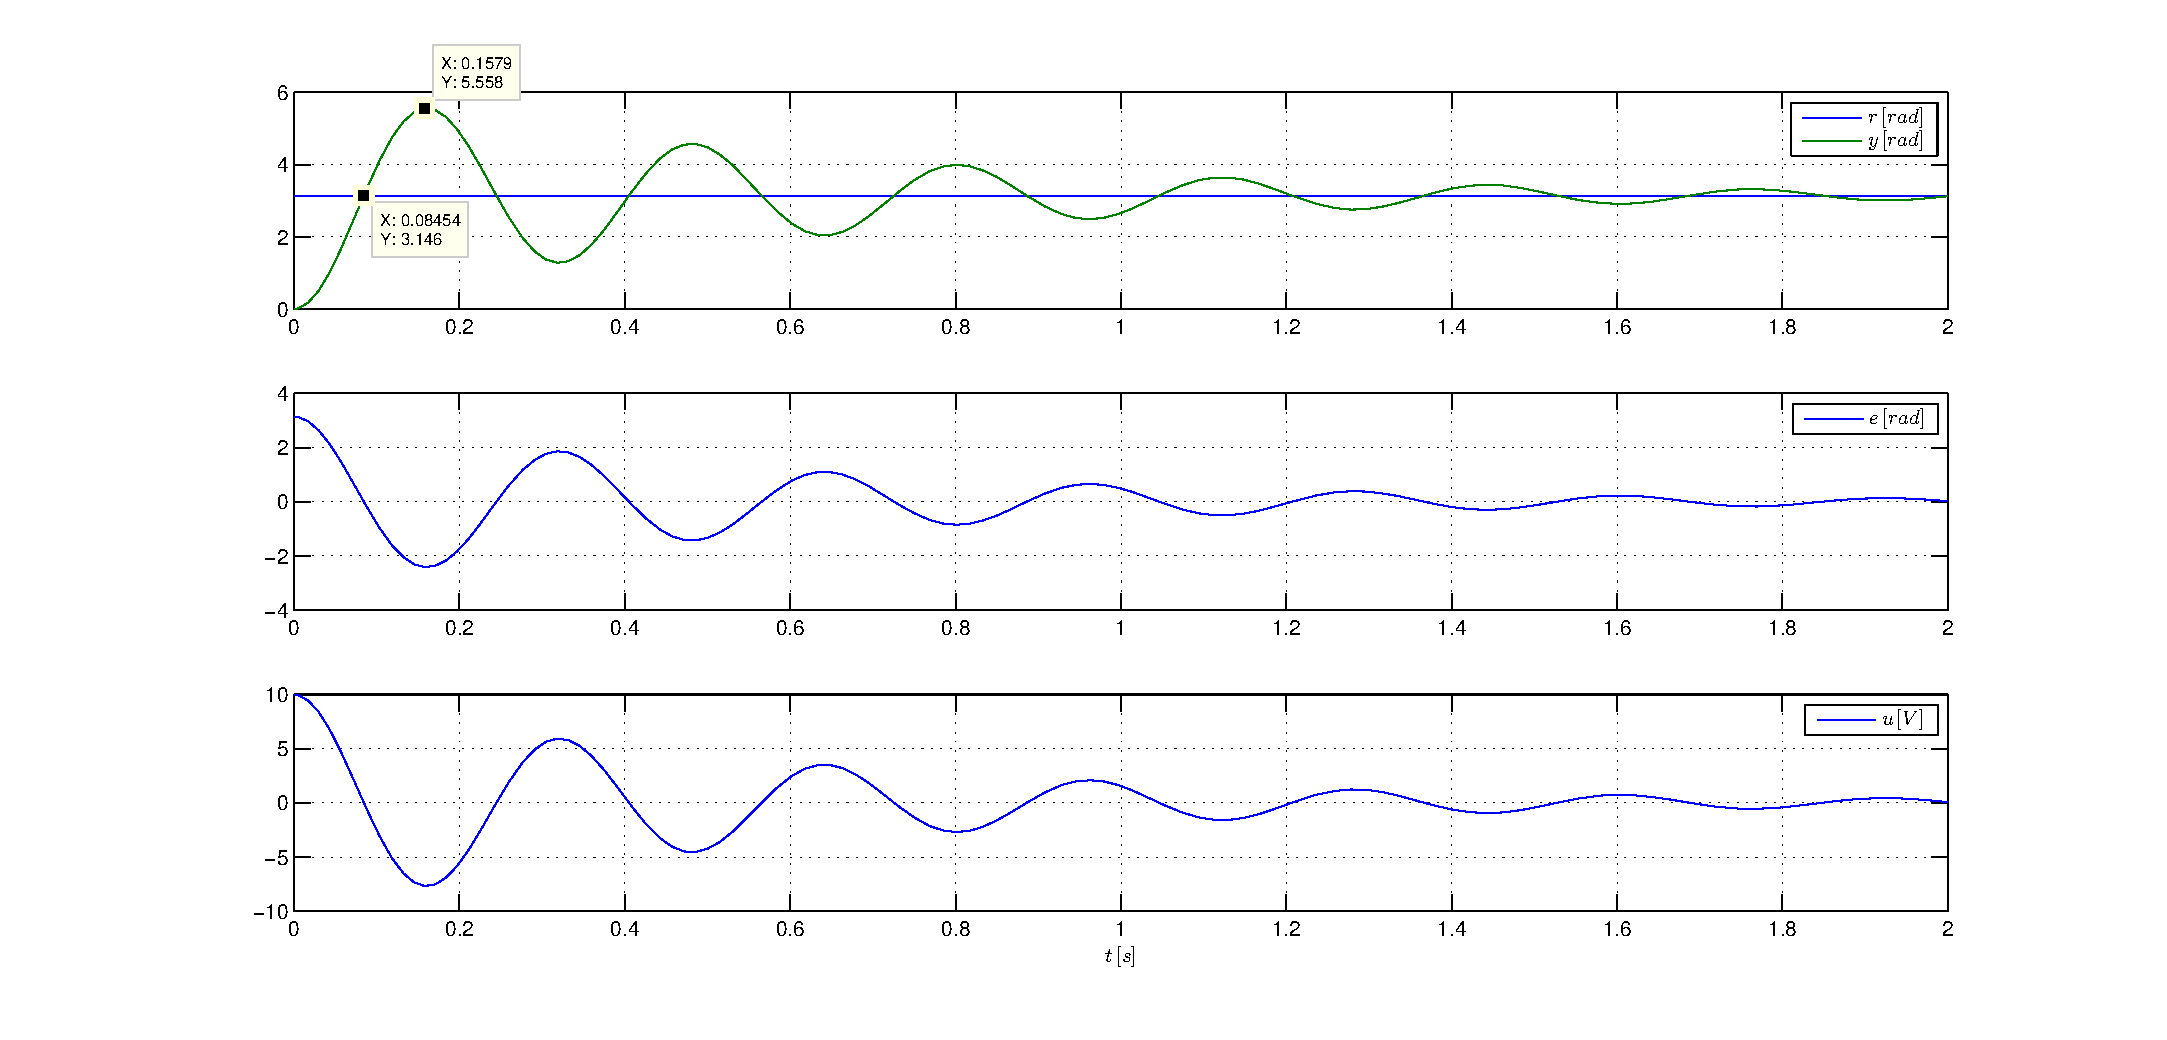
\includegraphics[width=1.0\textwidth]{img/sim.eps}
	\caption{Respuesta temporal en simulación del sistema en lazo cerrado con $K_p=3.18$ para $r=\pi\ [rad]$.}
	\label{fig:sim}
\end{figure}

\begin{figure}[H]
	\centering
		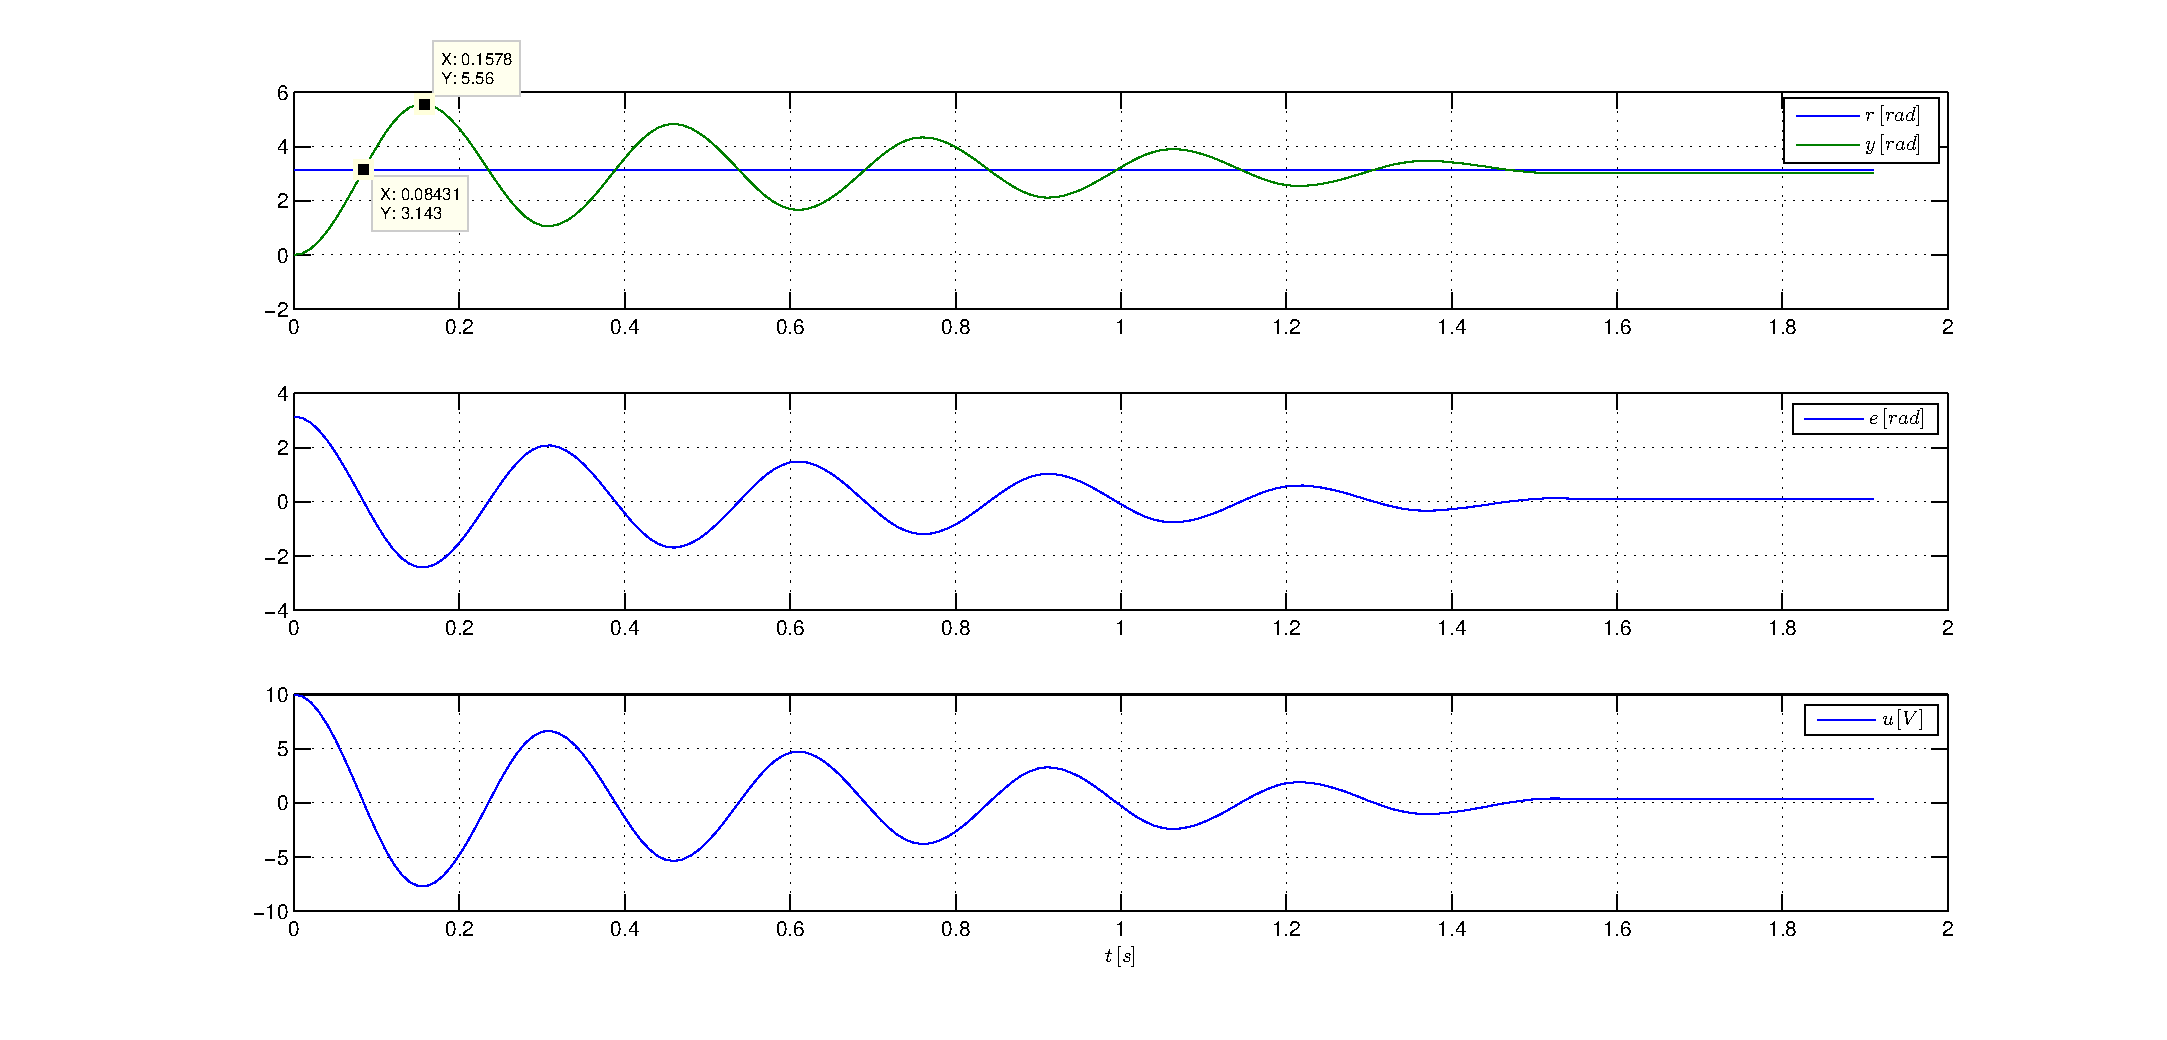
\includegraphics[width=1.0\textwidth]{img/exp.eps}
	\caption{Respuesta temporal experimental del sistema en lazo cerrado con $K_p=3.18$ para $r=\pi\ [rad]$.}
	\label{fig:exp}
\end{figure}

Para tener derecho a examen ordinario es necesario tener el $80\left[\%\right]$ de asistencia \citep{urlREUAQ2026}.

Cada miembro del equipo (en orden alfabético tal y como aparecen en la portada del reporte) discute los resultados.

\subsection{Arvizu Pérez Pedro}
En la Figura...

\subsection{Barrera López Daniel}
En la Figura...

\subsection{Galicia Rocha Sandra}
En la Figura...

\subsection{Mateos Rico Juan Carlos}
En la Figura...
 
\subsection{Resultados y discusión del equipo}

Se escribe la discusión de los resultados de manera colectiva o del equipo. En la Figura \ref{fig:sim} se puede observar en simulación un tiempo de levantamiento $t_r=0.08454\ [s]$ y un sobrepaso $M_p=76.92\ [\%]$ mientras que de manera experimental (ver Figura \ref{fig:exp}) se obtuvo un tiempo de levantamiento $t_r=0.08431\ [s]$ y un sobrepaso $M_p=76.98\ [\%]$.



\section{Conclusiones}
Cada miembro del equipo (en orden alfabético tal y como aparecen en la portada del reporte) escribe sus conclusiones.

\subsection{Arvizu Pérez Pedro}
En esta práctica...
 

\subsection{Barrera López Daniel}
En esta práctica...

\subsection{Galicia Rocha Sandra}
En esta práctica...

\subsection{Mateos Rico Juan Carlos}
 En esta práctica...
 
\subsection{Conclusiones del equipo}
Se escriben las conclusiones colectivas o del equipo. En esta práctica...




\vspace{10 mm}
\addcontentsline{toc}{section}{Bibliografía}
\bibliographystyle{uaq_prev}%{uaq_prev}%{apalike}%{apsr}%{apalike}%{abbrvnat}%archivo .bst
\bibliography{rep}%archivo .bib

\newpage
\section{Anexos}

\subsection{Programa para graficar la simulación}\label{proggsim}
En este anexo se muestra el código fuente para graficar los resultados en simulación con el intérprete de LaTeX.
{\scriptsize
\begin{verbatim}
%Gráfica del control de posición
clc;
clear all;
close all;
%leyendo las muestras tomadas al sistema
fid=fopen('gsim.txt','r'); %gsim simulación, gexp experimento
datos=fscanf(fid, '%f', [5 inf]);    % datos tiene 5 renglones
fclose(fid);
t=datos(1,:); 
r=datos(2,:);
y=datos(3,:);
u=datos(4,:);
e=datos(5,:);

figure(1)
subplot(3,1,1)
plot(t,r,t,y);
set(legend('$r\left[rad\right]$','$y\left[rad\right]$'), 'interpreter', 'latex')
grid on;

subplot(3,1,2)
plot(t,e);
set(legend('$e\left[rad\right]$'), 'interpreter', 'latex')
grid on;

subplot(3,1,3)
plot(t,u);
set(legend('$u\left[V\right]$'), 'interpreter', 'latex')
xlabel('$t\left[s\right]$', 'interpreter', 'latex')
grid on;
\end{verbatim}
}

\subsection{Programa para graficar la experimentación}
En este anexo se muestra el código fuente para graficar los resultados experimentales con el intérprete de LaTeX.
{\scriptsize
\begin{verbatim}
%Gráfica del control de posición
clc;
clear all;
close all;
%leyendo las muestras tomadas al sistema
fid=fopen('gexp.txt','r'); %gsim simulación, gexp experimento
datos=fscanf(fid, '%f', [5 inf]);    % datos tiene 5 renglones
fclose(fid);
t=datos(1,:); 
r=datos(2,:);
y=datos(3,:);
u=datos(4,:);
e=datos(5,:);

figure(1)
subplot(3,1,1)
plot(t,r,t,y);
set(legend('$r\left[rad\right]$','$y\left[rad\right]$'), 'interpreter', 'latex')
grid on;

subplot(3,1,2)
plot(t,e);
set(legend('$e\left[rad\right]$'), 'interpreter', 'latex')
grid on;

subplot(3,1,3)
plot(t,u);
set(legend('$u\left[V\right]$'), 'interpreter', 'latex')
xlabel('$t\left[s\right]$', 'interpreter', 'latex')
grid on;
\end{verbatim}
}



\end{document}